\documentclass{article}
\usepackage[utf8]{inputenc}

\usepackage{graphicx}
\usepackage{subcaption}

\usepackage{ifxetex}
\ifxetex
  \usepackage{fontspec}
\else
  \usepackage[T1]{fontenc}
  \usepackage[utf8]{inputenc}
  \usepackage{lmodern}
\fi

\title{Reporte de Actividad 7}
\author{Roberto Benard Orci}
\date{24/03/2018}

\begin{document}
\maketitle

\section{Síntesis}

En esta actividad usamos el artículo de Temple Fay y Sarah Graham sobre las ecuaciones de resortes acoplados para modelar el movimiento de dos resortes acoplados, colgados en serie desde el techo. Usamos un modelo lineal, que utiliza la Ley de Hooke, un modelo no lineal, y uno con fuerzas, el movimiento de cada peso se describe por una ecuación diferencial diferente..

\vspace{0.3cm}

Las soluciones obtenidas producen una amplia variedad de movimientos, el modelo es adecuado para practicar el modelamiento de ecuaciones diferenciales con herramientas de computo. 

\subsection*{Introducción}

Tenemos dos resortes y dos pesos unidos en serie, colgando del techo. Bajo el supuesto de que las fuerzas de restauración se comportan de acuerdo con Ley de Hooke, este problema de dos grados de libertad está modelado por un par de ecuaciones diferenciales lineales. Conforme avanzamos en este archivo, la Ley de Hooke no es suficiente y agregamos componentes a las ecuaciones.

\vspace{0.3cm}

Mediante diferentes ejemplos, podemos observar que pequeños cambios en las condiciones iniciales pueden generar cambios significativos en el movimiento de los resortes, movimientos que pueden ser analizados mediante diferentes gráficas.

\subsection*{El modelo de resorte acoplado}

El modelo consiste en dos resortes y dos pesos, el primer resorte tiene una constante \textit{k1}, este se adjunta al techo y un peso de masa \textit{m1} está unido al extremo inferior del resorte. A este peso, se le agrega un segundo resorte con constante \textit{k2}, adjunto a este se encuentra un peso de masa \textit{m2}.

\vspace{0.3cm}

Cuando el sistema permanece en equilibrio, medimos el desplazamiento de cada peso \textit{l1} y \textit{l2}. Lo que mediremos serán las posiciones, \textit{x1(t)} y \textit{x2(t)}, que cambiaran con respecto al tiempo.

\begin{center}
	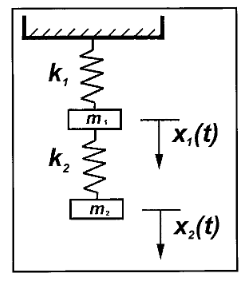
\includegraphics[width=4cm]{ModeloResortesAcoplados.png}
 
\end{center}
\vspace{0.3cm}

Se modelan varios ejemplos, en los cuales se considera que \textit{m1 = m2 = 1}. Cada uno de estos ejemplos tiene diferentes parametros, o diferentes condiciones iniciales.

\section{Ejemplo Base}

Para poder graficar todos los ejemplos usamos como base el código de \textit{Coupled spring-mass system}, en el cual aparecía el siguiente código:

\begin{verbatim}
def vectorfield(w, t, p):

    x1, y1, x2, y2 = w
    m1, m2, k1, k2, L1, L2, b1, b2 = p

    # Create f = (x1',y1',x2',y2'):
    f = [y1,
         (-b1 * y1 - k1 * (x1 - L1) + k2 * (x2 - x1 - L2)) / m1,
         y2,
         (-b2 * y2 - k2 * (x2 - x1 - L2)) / m2]
    return f
\end{verbatim}

En esta sección de código se definen diferentes vectores, los cuales tendrán diferentes valores de acuerdo a los parámetros que tienen, y la forma de las ecuaciones diferenciales.

\vspace{0.6cm}

\begin{verbatim}
from scipy.integrate import odeint

# Parameter values
# Masses:
m1 = 1.0
m2 = 1.5
# Spring constants
k1 = 8.0
k2 = 40.0
# Natural lengths
L1 = 0.5
L2 = 1.0
# Friction coefficients
b1 = 0.8
b2 = 0.5

# Initial conditions
# x1 and x2 are the initial displacements; y1 and y2 are the initial velocities
x1 = 0.5
y1 = 0.0
x2 = 2.25
y2 = 0.0

# ODE solver parameters
abserr = 1.0e-8
relerr = 1.0e-6
stoptime = 10.0
numpoints = 250

# Create the time samples for the output of the ODE solver.
# I use a large number of points, only because I want to make
# a plot of the solution that looks nice.
t = [stoptime * float(i) / (numpoints - 1) for i in range(numpoints)]

# Pack up the parameters and initial conditions:
p = [m1, m2, k1, k2, L1, L2, b1, b2]
w0 = [x1, y1, x2, y2]

# Call the ODE solver.
wsol = odeint(vectorfield, w0, t, args=(p,),
              atol=abserr, rtol=relerr)

with open('two-springs.dat', 'w') as f:
    # Print & save the solution.
    for t1, w1 in zip(t, wsol):
        print >> f, t1, w1[0], w1[1], w1[2], w1[3]
\end{verbatim}

En esta otra sección de código se  les da un valor a todos los parámetros, se definen los valores mínimos de los errores de los cálculos, y el número de puntos que se graficaran en un cierto intervalo de tiempo. Luego, con ayuda de \textit{ODEINT} se resuelven las ecuaciones diferenciales que se definieron en la sección de código anterior con los valores que se acaban de establecer, y se guarda una gran lista de datos en el archivo \textit{two-springs.dat}.

\vspace{0.6cm}

\begin{verbatim}
from numpy import loadtxt
from pylab import figure, plot, xlabel, grid, hold, legend, title, savefig
from matplotlib.font_manager import FontProperties

t, x1, xy, x2, y2 = loadtxt('two-springs.dat', unpack=True)

figure(1, figsize=(6, 4.5))

xlabel('t')
grid(True)
hold(True)
lw = 1

plot(t, x1, 'b', linewidth=lw)
plot(t, x2, 'g', linewidth=lw)

legend((r'$x_1$', r'$x_2$'), prop=FontProperties(size=16))
title('Mass Displacements for the\nCoupled Spring-Mass System')
savefig('two_springs.png', dpi=100
\end{verbatim}

Por ultimo, se usa el archivo de datos que se genero en la sección de código anterior para graficar diferentes parámetros. En este ejemplo se graficaron los valores de las posiciones \textit{x1} y \textit{x2} con respecto al tiempo.

\begin{center}
	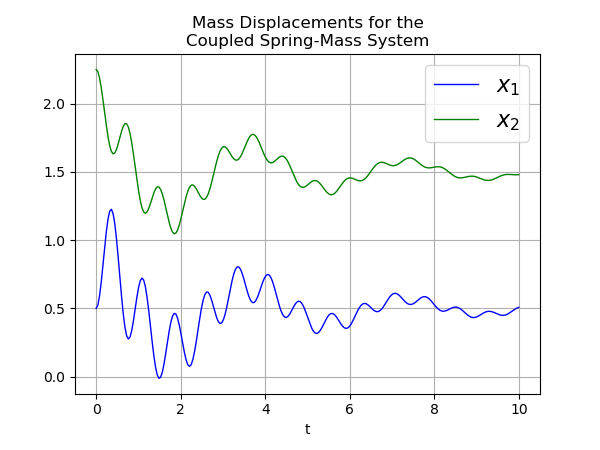
\includegraphics[width=6cm]{two_springs.png}
 
\end{center}
\vspace{0.3cm}

\section{Resultados}

Cada uno de estos ejemplos es distinto del anterior de alguna manera. Los ejemplos \textit{2} utilizan la Ley de Hooke, a los ejemplos \textit{3} se les agrega una componente no lineal a sus ecuaciones, y a los ejemplos \textit{4} se les agrega una componente a las ecuaciones que representa una fuerza externa afectando a los resortes.

\subsection*{Ejemplo 2.1}

La figura \textit{(a)} representa a \textit{x1} y \textit{x2} con respecto al tiempo. La figura \textit{(b)} representa a \textit{x1} y \textit{x2} con respecto a \textit{v1} y \textit{v2} respectivamente. La figura \textit{(c)} representa a \textit{x1} con respecto a \textit{x2}.
Finalmente, las figuras \textit{(d)} y \textit{(e)} representan los errores relativos de los resultados de las ecuaciones contra los valores verdaderos de la posición con respecto al tiempo.

\begin{figure}[h!]
  \centering
  \begin{subfigure}[b]{0.32\linewidth}
    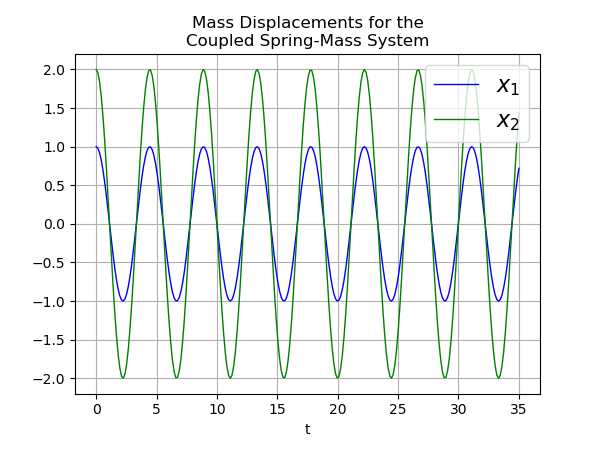
\includegraphics[width=\linewidth]{two_springs211.png}
     \caption{}
  \end{subfigure}
  \begin{subfigure}[b]{0.32\linewidth}
    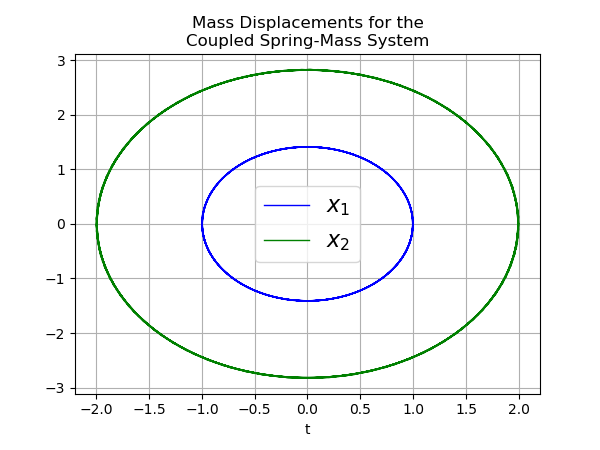
\includegraphics[width=\linewidth]{two_springs212.png}
    \caption{}
  \end{subfigure}
  \begin{subfigure}[b]{0.32\linewidth}
    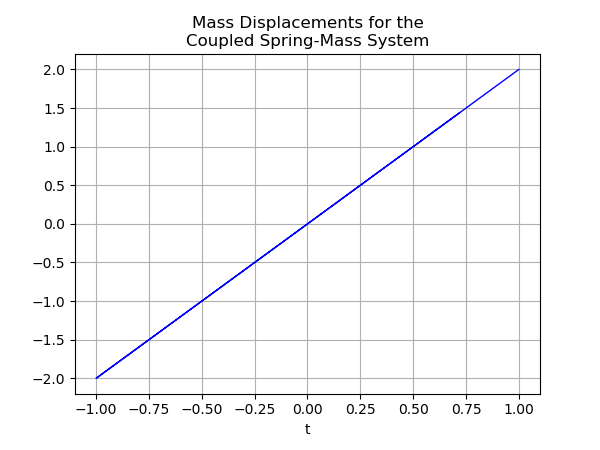
\includegraphics[width=\linewidth]{two_springs213.png}
    \caption{}
  \end{subfigure}
  \begin{subfigure}[b]{0.45\linewidth}
    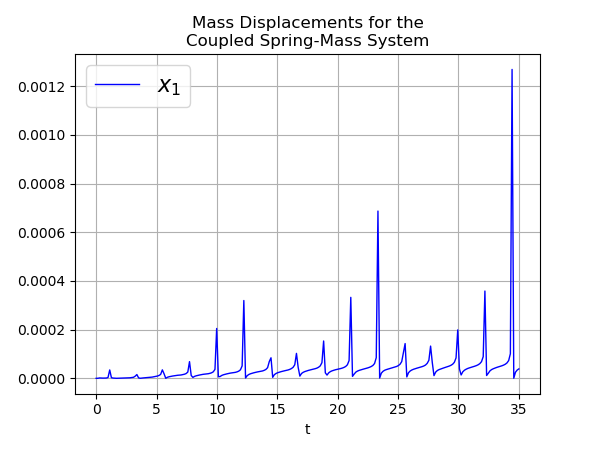
\includegraphics[width=\linewidth]{two_springs21e1.png}
    \caption{}
  \end{subfigure}
  \begin{subfigure}[b]{0.45\linewidth}
    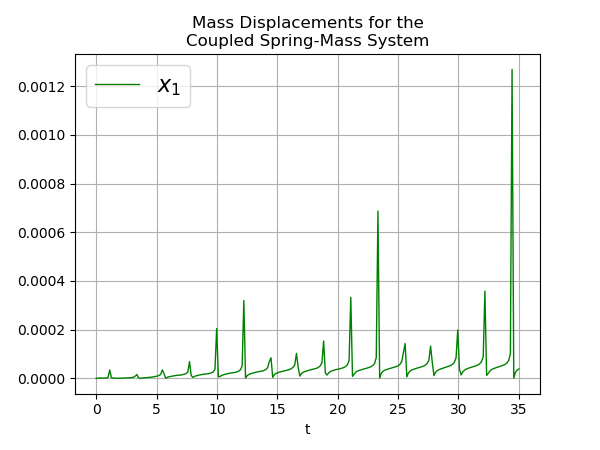
\includegraphics[width=\linewidth]{two_springs21e2.png}
    \caption{}
  \end{subfigure}
\end{figure}

Estas dos ultimas gráficas fueron hechas agregando esto a la segunda sección de código:

\begin{verbatim}
print(t1, w1[0], w1[1], w1[2], w1[3], np.abs((w1[0]-(np.cos(np.sqrt(2.0)
*t1)))/(np.cos(np.sqrt(2.0)*t1))), np.abs((w1[2]-(2.0*np.cos(np.sqrt(2.
0)*t1)))/(2.0*np.cos(np.sqrt(2.0)*t1))),file=f)
\end{verbatim}

Y esto a la tercera sección de código:

\begin{verbatim}
t, x1, xy, x2, y2, e1, e2 = loadtxt('two_springs21.dat', unpack=True)
\end{verbatim}

Donde \textit{e1} y \textit{e2} son las listas de los valores de los errores relativos con respecto al tiempo.

\vspace{5cm}

\subsection*{Ejemplo 2.2}

\begin{figure}[h!]
  \centering
  \begin{subfigure}[b]{0.32\linewidth}
    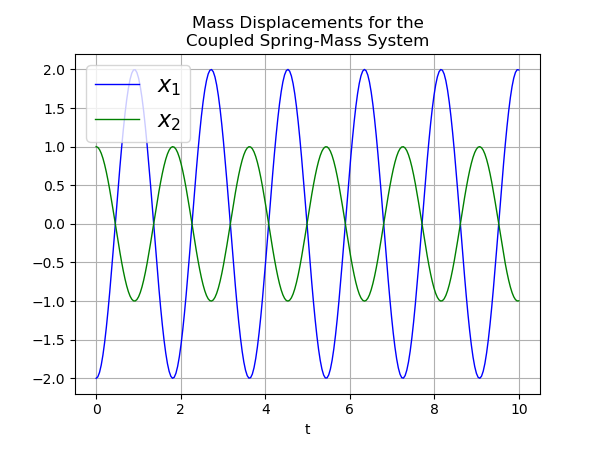
\includegraphics[width=\linewidth]{two_springs221.png}
     \caption{}
  \end{subfigure}
  \begin{subfigure}[b]{0.32\linewidth}
    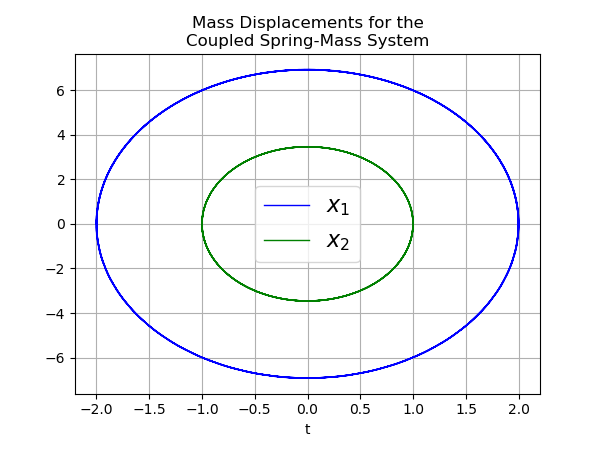
\includegraphics[width=\linewidth]{two_springs222.png}
    \caption{}
  \end{subfigure}
  \begin{subfigure}[b]{0.32\linewidth}
    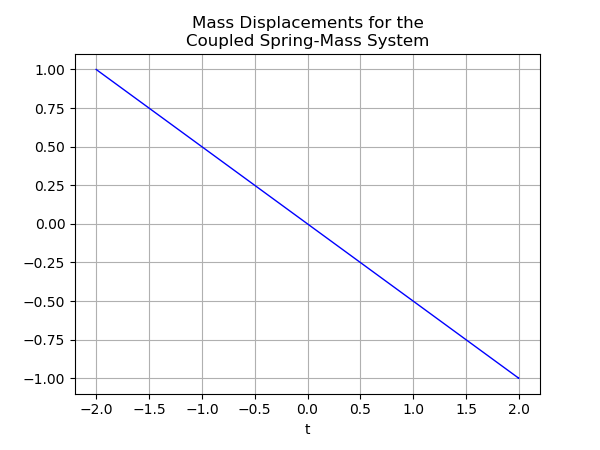
\includegraphics[width=\linewidth]{two_springs223.png}
    \caption{}
  \end{subfigure}
  \begin{subfigure}[b]{0.45\linewidth}
    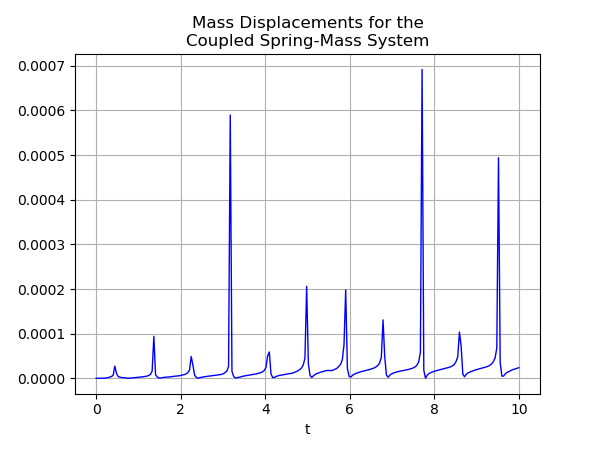
\includegraphics[width=\linewidth]{two_springs22e1.png}
    \caption{}
  \end{subfigure}
  \begin{subfigure}[b]{0.45\linewidth}
    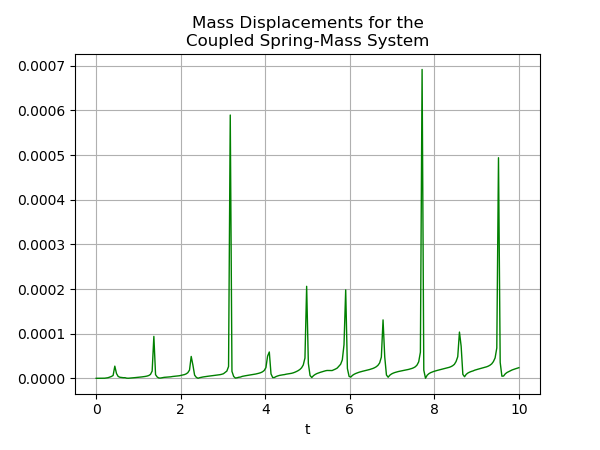
\includegraphics[width=\linewidth]{two_springs22e2.png}
    \caption{}
  \end{subfigure}
\end{figure}

Cada una de estas gráficas representa lo mismo que en el ejemplo anterior solo que con diferentes parámetros. De igual manera, se agregaron las mismas cosas al código, solo que con las diferencias respectivas de los valores verdaderos de los errores.

\vspace{6.5cm}

\subsection*{Ejemplo 2.3}

En este ejemplo y en el siguiente no es posible calcular los errores. La figura \textit{(a)} representa a \textit{x1} y \textit{x2} con respecto al tiempo, pero a diferencia de los anteriores, las figuras \textit{(b)} y \textit{(c)} muestran a \textit{x1} y \textit{x2} respectivamente, con respecto al tiempo, para poder visualizar mejor lo que esta pasando. De la misma manera, las figuras \textit{(d)} y \textit{(e)} muestran a \textit{x1} y \textit{x2} con respecto a \textit{v1} y \textit{v2} respectivamente. Finalmente, la figura \textit{(f)} representa a \textit{x1} con respecto a \textit{x2}.

\begin{figure}[h!]
  \centering
  \begin{subfigure}[b]{0.32\linewidth}
    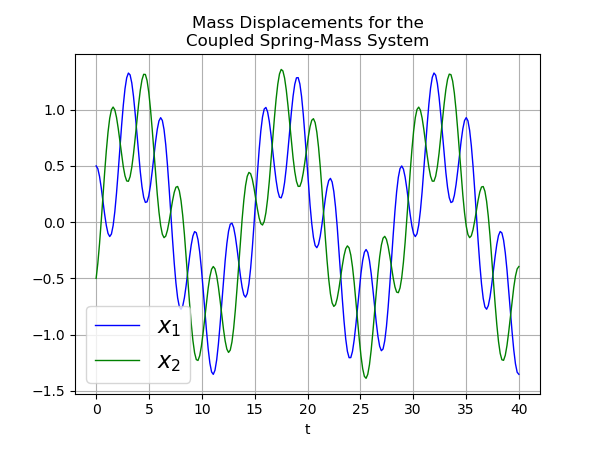
\includegraphics[width=\linewidth]{two_springs231.png}
     \caption{}
  \end{subfigure}
  \begin{subfigure}[b]{0.32\linewidth}
    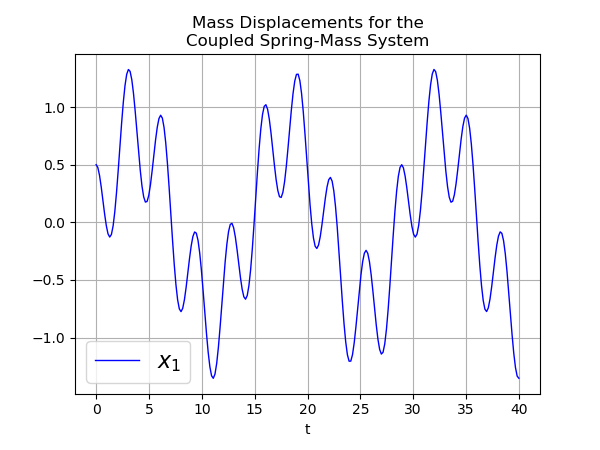
\includegraphics[width=\linewidth]{two_springs232.png}
    \caption{}
  \end{subfigure}
  \begin{subfigure}[b]{0.32\linewidth}
    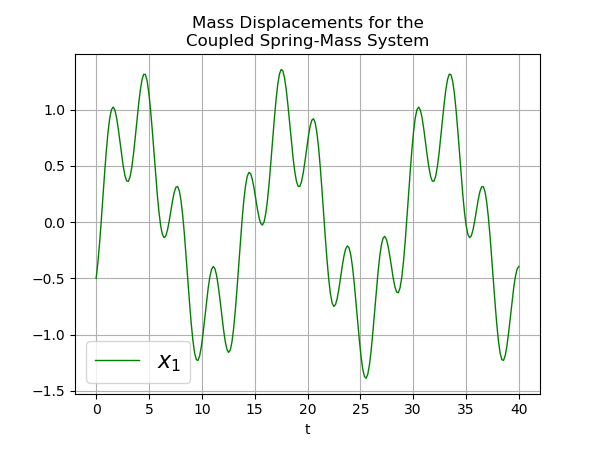
\includegraphics[width=\linewidth]{two_springs233.png}
    \caption{}
  \end{subfigure}
  \begin{subfigure}[b]{0.45\linewidth}
    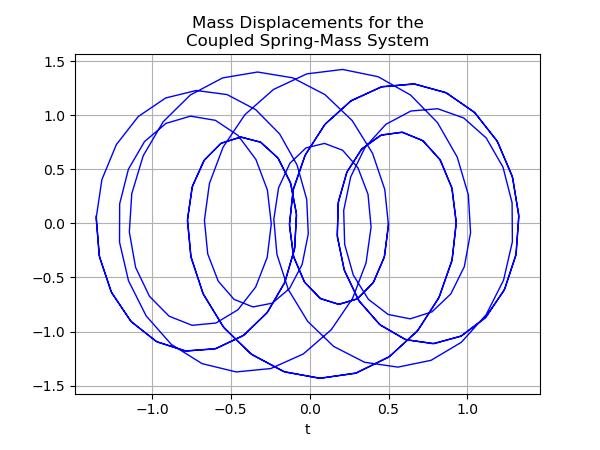
\includegraphics[width=\linewidth]{two_springs234.png}
    \caption{}
  \end{subfigure}
  \begin{subfigure}[b]{0.45\linewidth}
    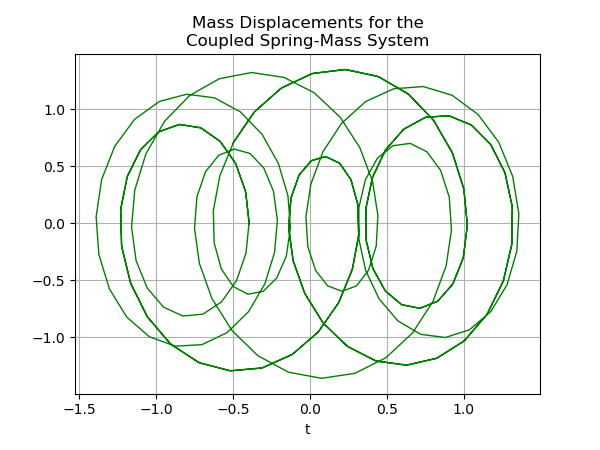
\includegraphics[width=\linewidth]{two_springs235.png}
    \caption{}
  \end{subfigure}
  \begin{subfigure}[b]{0.5\linewidth}
    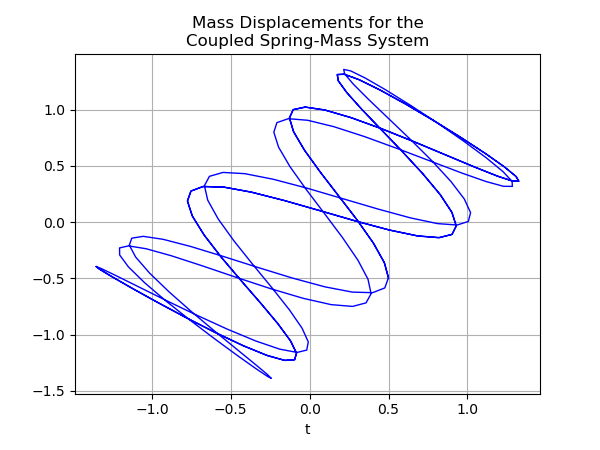
\includegraphics[width=\linewidth]{two_springs236.png}
    \caption{}
  \end{subfigure}
\end{figure}

\vspace{1.5cm}

\subsection*{Ejemplo 2.4}

Cada una de estas gráficas representa lo mismo que en el ejemplo anterior solo que con diferentes parámetros. En este ejemplo se implemento la fricción, por lo que se puede ver en las gráficas que el movimiento se va haciendo cada vez mas pequeño.

\begin{figure}[h!]
  \centering
  \begin{subfigure}[b]{0.32\linewidth}
    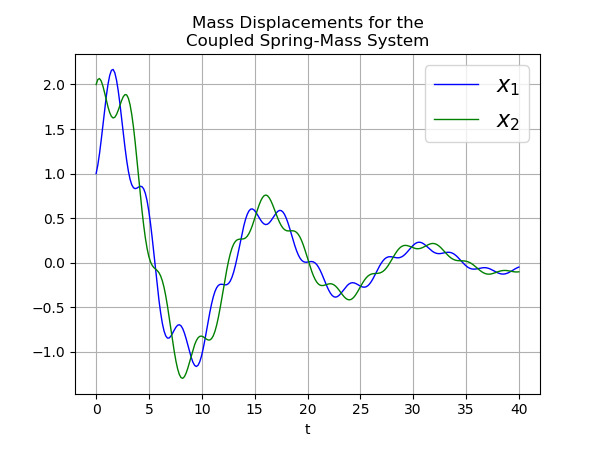
\includegraphics[width=\linewidth]{two_springs241.png}
     \caption{}
  \end{subfigure}
  \begin{subfigure}[b]{0.32\linewidth}
    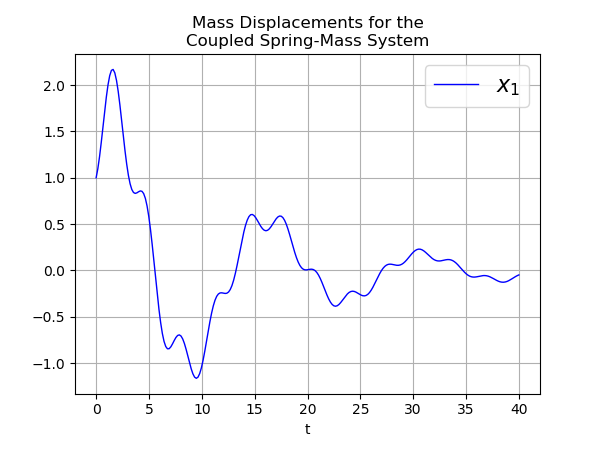
\includegraphics[width=\linewidth]{two_springs242.png}
    \caption{}
  \end{subfigure}
  \begin{subfigure}[b]{0.32\linewidth}
    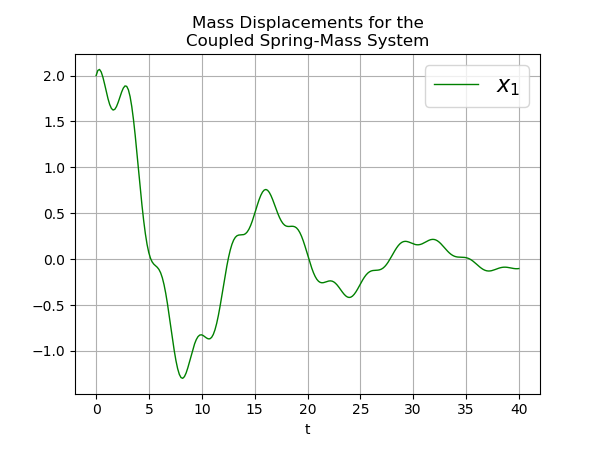
\includegraphics[width=\linewidth]{two_springs243.png}
    \caption{}
  \end{subfigure}
  \begin{subfigure}[b]{0.45\linewidth}
    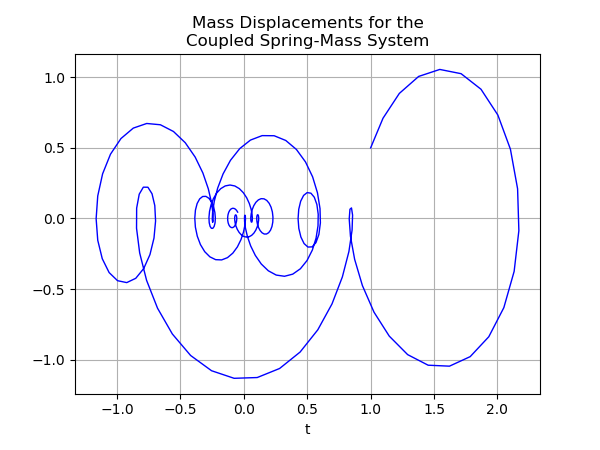
\includegraphics[width=\linewidth]{two_springs244.png}
    \caption{}
  \end{subfigure}
  \begin{subfigure}[b]{0.45\linewidth}
    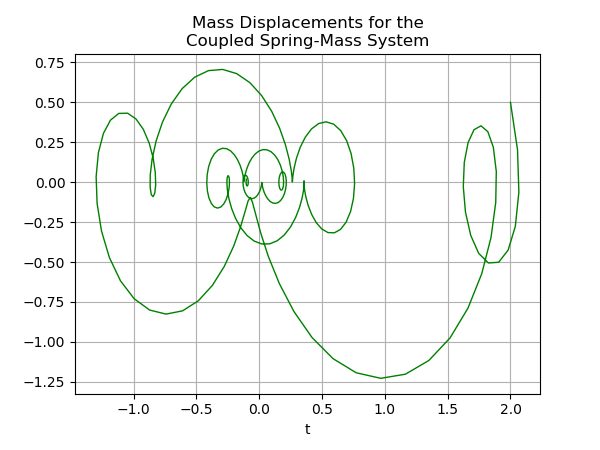
\includegraphics[width=\linewidth]{two_springs245.png}
    \caption{}
  \end{subfigure}
  \begin{subfigure}[b]{0.5\linewidth}
    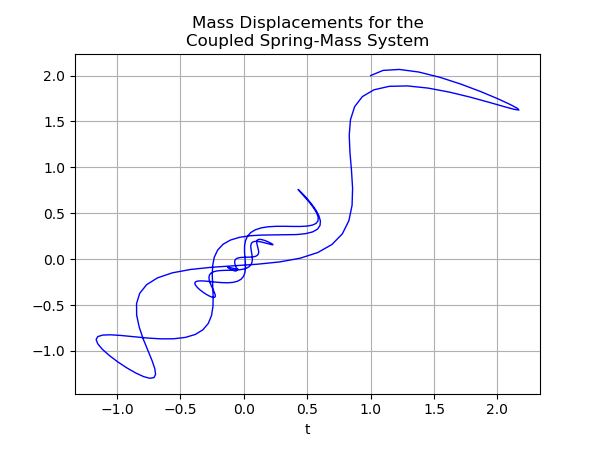
\includegraphics[width=\linewidth]{two_springs246.png}
    \caption{}
  \end{subfigure}
\end{figure}

\vspace{1.5cm}

\subsection*{Ejemplo 3.1}

Cada una de estas gráficas representa lo mismo que en el ejemplo anterior solo que ahora se implementa un elemento a las ecuaciones para que no sean lineales.

\begin{verbatim}
    f = [y1,
         (-b1 * y1 - k1 * (x1 - L1) + k2 * (x2 - x1 - L2) + u1 * x1**3 + u2 * 
         (x1 - x2)**3) / m1,
         y2,
         (-b2 * y2 - k2 * (x2 - x1 - L2) + u2 * (x2 - x1)**3) / m2]
    return f
\end{verbatim}

\begin{figure}[h!]
  \centering
  \begin{subfigure}[b]{0.32\linewidth}
    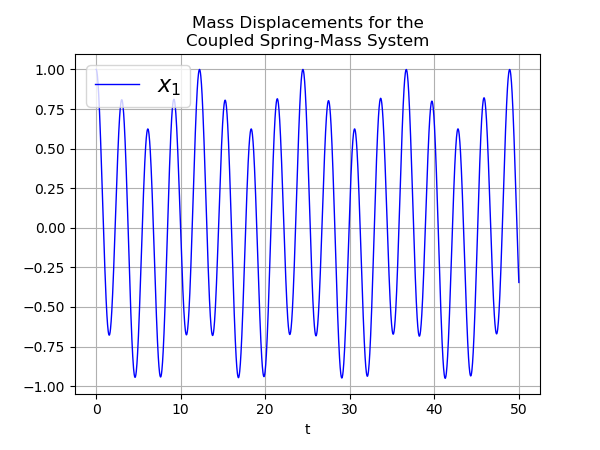
\includegraphics[width=\linewidth]{two_springs311.png}
     \caption{}
  \end{subfigure}
  \begin{subfigure}[b]{0.32\linewidth}
    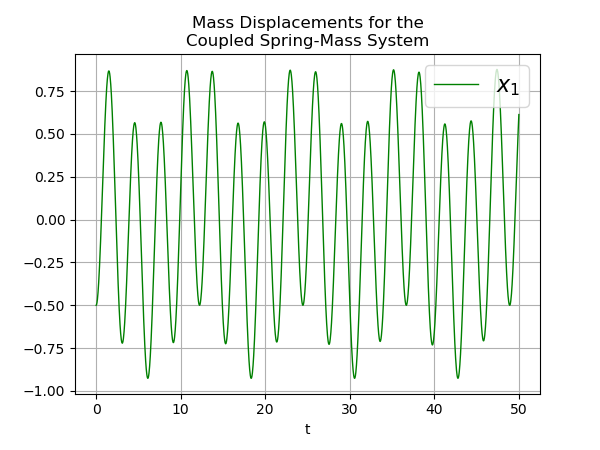
\includegraphics[width=\linewidth]{two_springs312.png}
    \caption{}
  \end{subfigure}
  \begin{subfigure}[b]{0.32\linewidth}
    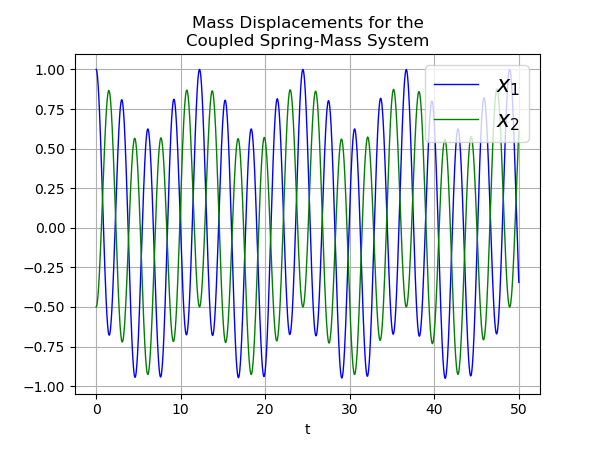
\includegraphics[width=\linewidth]{two_springs315.png}
    \caption{}
  \end{subfigure}
  \begin{subfigure}[b]{0.45\linewidth}
    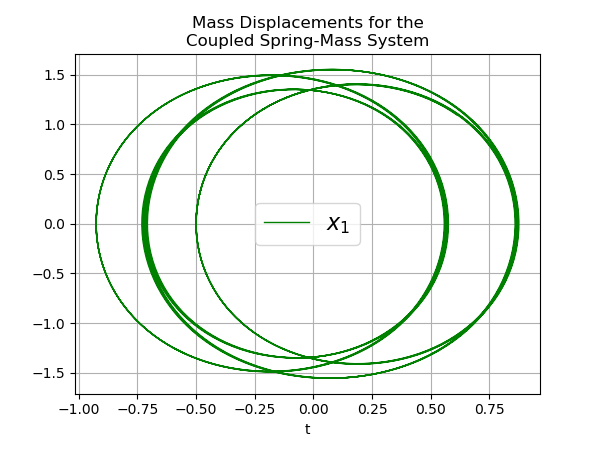
\includegraphics[width=\linewidth]{two_springs314.png}
    \caption{}
  \end{subfigure}
  \begin{subfigure}[b]{0.45\linewidth}
    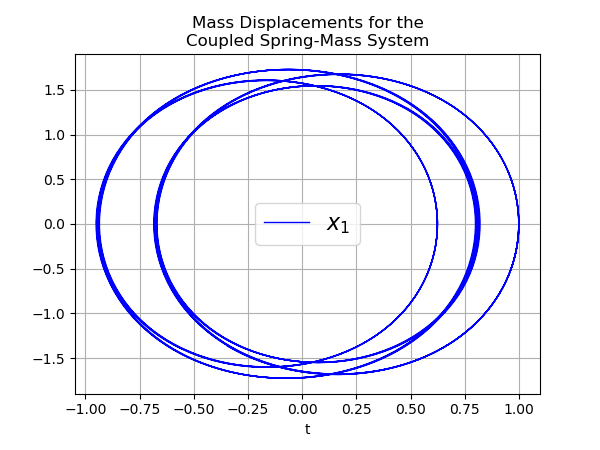
\includegraphics[width=\linewidth]{two_springs313.png}
    \caption{}
  \end{subfigure}
  \begin{subfigure}[b]{0.5\linewidth}
    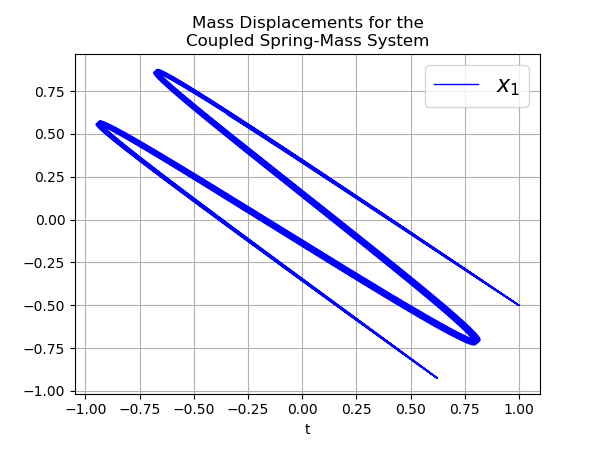
\includegraphics[width=\linewidth]{two_springs316.png}
    \caption{}
  \end{subfigure}
\end{figure}



\subsection*{Ejemplo 3.2}

Estas gráficas son las mismas que las gráficas \textit{(d)}, \textit{(e)}, y \textit{(f)} (mismos parámetros) solo que con condiciones iniciales diferentes.

\begin{figure}[h!]
  \centering
  \begin{subfigure}[b]{0.45\linewidth}
    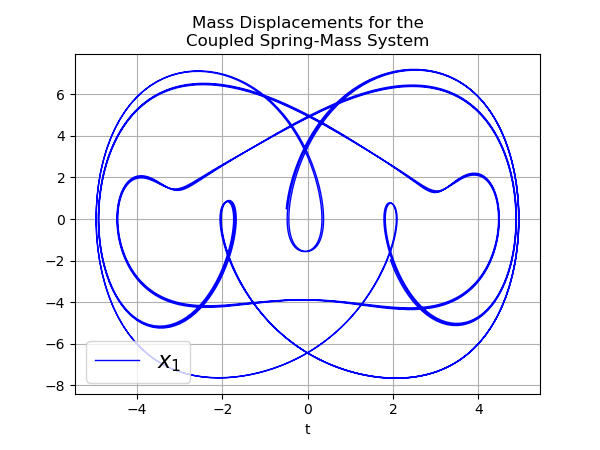
\includegraphics[width=\linewidth]{two_springs321.png}
    \caption{}
  \end{subfigure}
  \begin{subfigure}[b]{0.45\linewidth}
    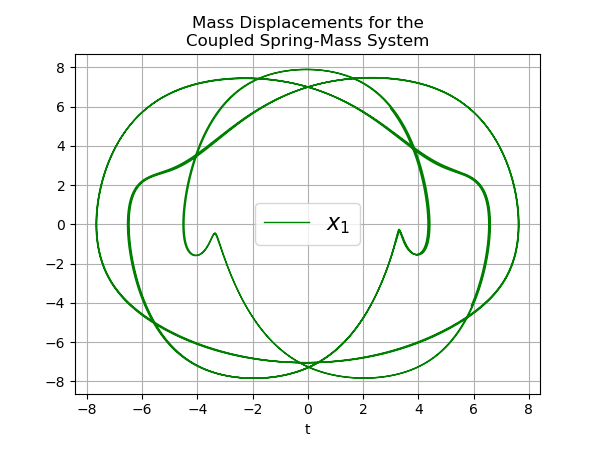
\includegraphics[width=\linewidth]{two_springs322.png}
    \caption{}
  \end{subfigure}
  \begin{subfigure}[b]{0.5\linewidth}
    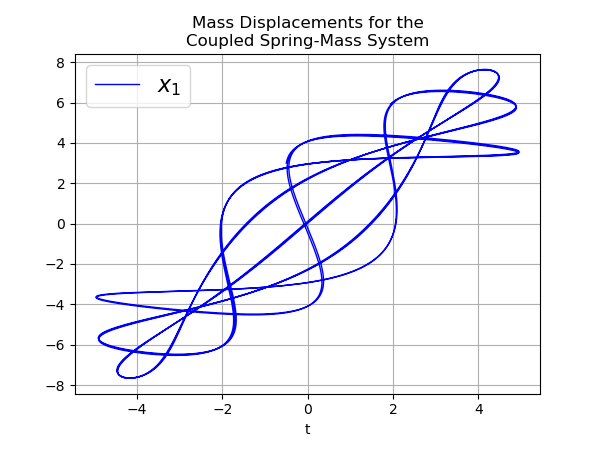
\includegraphics[width=\linewidth]{two_springs323.png}
    \caption{}
  \end{subfigure}
\end{figure}

\vspace{5.5cm}

\subsection*{Ejemplo 3.3}

Cada una de estas gráficas representa lo mismo que en el ejemplo anterior solo que con un cambio de 0.1 en la posición inicial de \textit{x1}, esto muestra como un pequeño cambio en cualquier parámetro puede afectar el movimiento de los resortes.

\begin{figure}[h!]
  \centering
  \begin{subfigure}[b]{0.45\linewidth}
    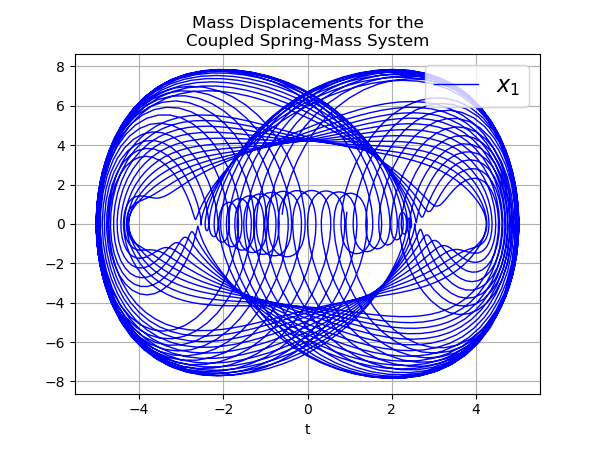
\includegraphics[width=\linewidth]{two_springs331.png}
    \caption{}
  \end{subfigure}
  \begin{subfigure}[b]{0.45\linewidth}
    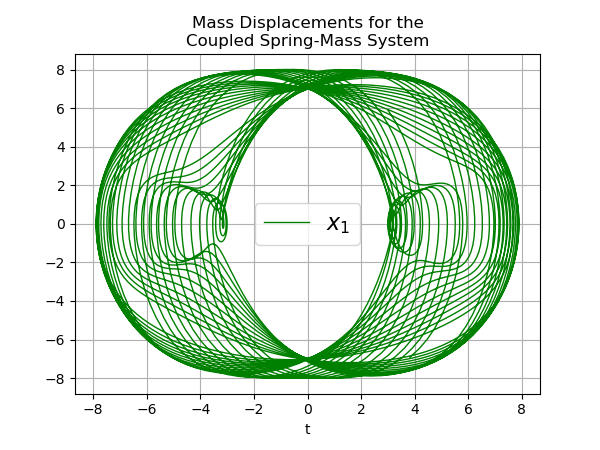
\includegraphics[width=\linewidth]{two_springs332.png}
    \caption{}
  \end{subfigure}
  \begin{subfigure}[b]{0.5\linewidth}
    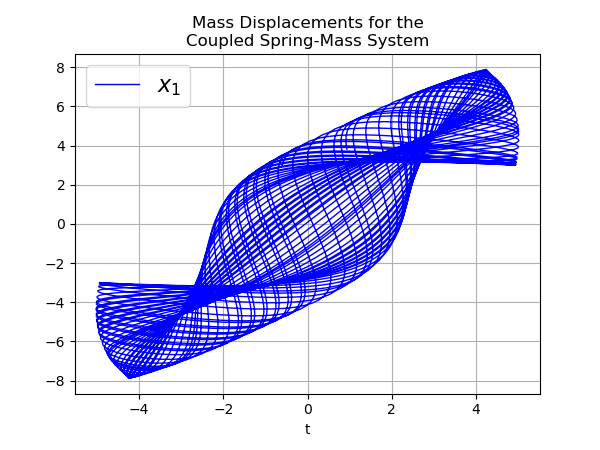
\includegraphics[width=\linewidth]{two_springs333.png}
    \caption{}
  \end{subfigure}
\end{figure}

\subsection*{Ejemplo 4.1}

En este ultimo ejemplo, no solo se le agregaron as partes no lineales del ejemplo 3, si no que también se le agregaron a las ecuaciones componentes de fuerzas externas.

\begin{verbatim}
		f = [y1,
         (-b1 * y1 - k1 * (x1 - L1) + k2 * (x2 - x1 - L2) + u1 * x1**3 + u2 * 
         (x1 - x2)**3 + F1 * np.cos(w1*t)) / m1,
         y2,
         (-b2 * y2 - k2 * (x2 - x1 - L2) + u2 * (x2 - x1)**3 + F2 * 
         np.cos(w2*t)) / m2]
    return f
\end{verbatim}

\begin{figure}[h!]
  \centering
  \begin{subfigure}[b]{0.45\linewidth}
    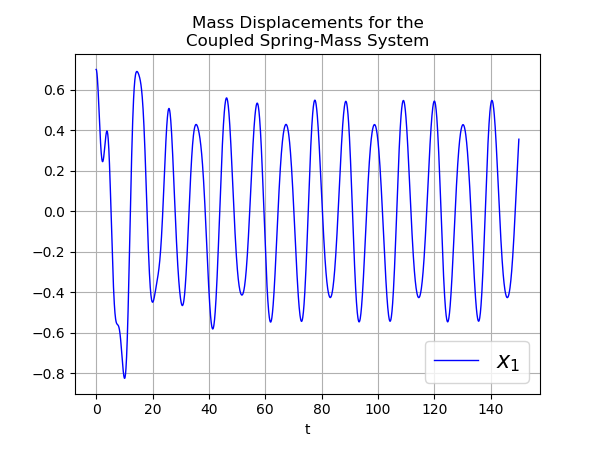
\includegraphics[width=\linewidth]{two_springs411.png}
     \caption{}
  \end{subfigure}
  \begin{subfigure}[b]{0.45\linewidth}
    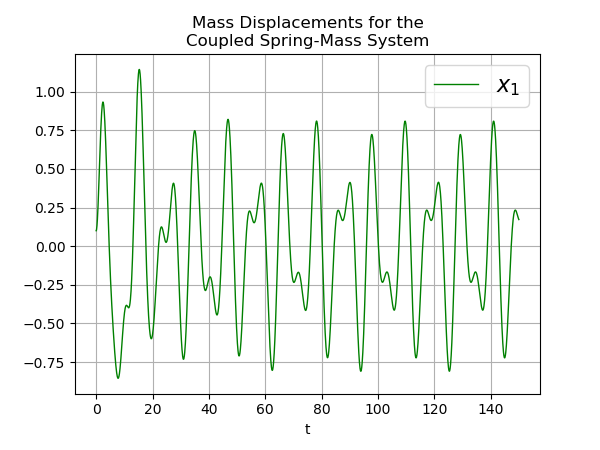
\includegraphics[width=\linewidth]{two_springs412.png}
    \caption{}
  \end{subfigure}
  \begin{subfigure}[b]{0.45\linewidth}
    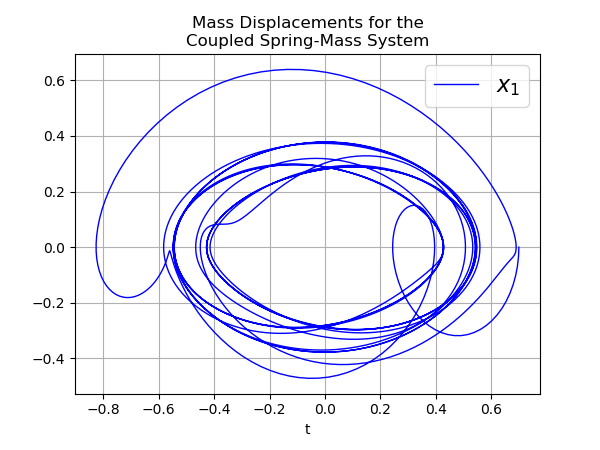
\includegraphics[width=\linewidth]{two_springs413.png}
    \caption{}
  \end{subfigure}
  \begin{subfigure}[b]{0.45\linewidth}
    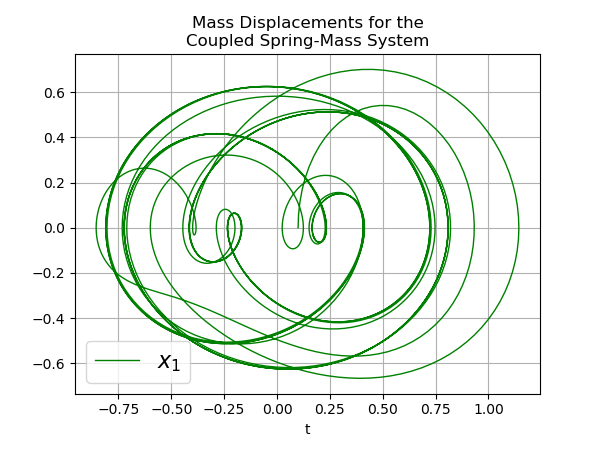
\includegraphics[width=\linewidth]{two_springs414.png}
    \caption{}
  \end{subfigure}
  \begin{subfigure}[b]{0.45\linewidth}
    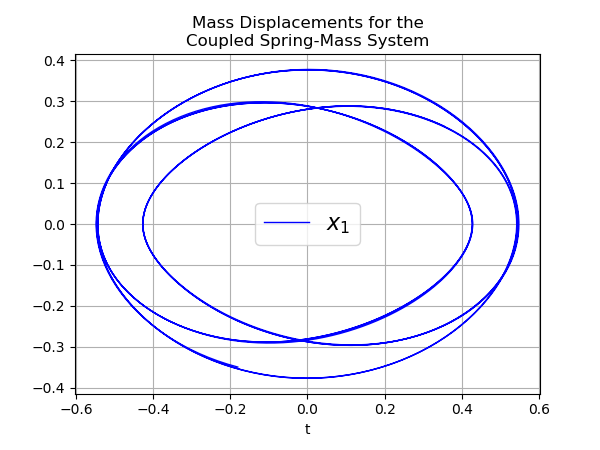
\includegraphics[width=\linewidth]{two_springs415.png}
    \caption{}
  \end{subfigure}
  \begin{subfigure}[b]{0.45\linewidth}
    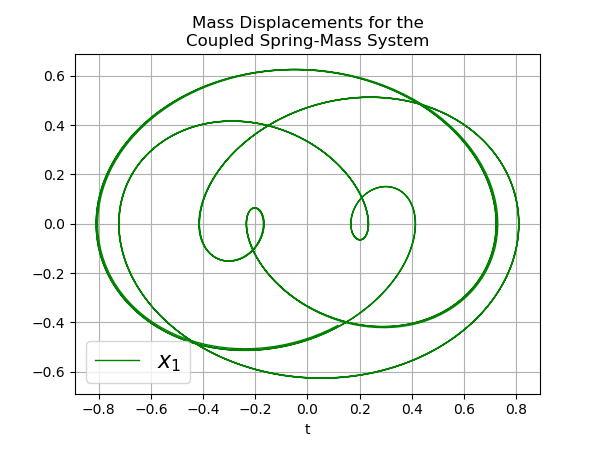
\includegraphics[width=\linewidth]{two_springs416.png}
    \caption{}
  \end{subfigure}
\end{figure}

Las figuras \textit{(a)} y \textit{(b)} representan a \textit{x1} y \textit{x2} con respecto al tiempo, respectivamente. Las figuras \textit{(c)} y \textit{(d)} representan a \textit{x1} y \textit{x2} con respecto a \textit{v1} y \textit{v2}, respectivamente. Por ultimo, las figuras \textit{(e)} y \textit{(f)} son las figuras \textit{(c)} y \textit{(d)} conforme el tiempo pasa, lo que significa que el movimiento de los resortes se estabilizara.

\vspace{1.0cm}

\section{Conclusiones}

Al terminar todos los ejemplos, uno puede apreciar lo útiles que son las herramientas de computo para modelar ecuaciones diferenciales. Al modelar todos los ejemplos, podemos ver que estos producen una amplia variedad de movimientos, cualquier cambio en las condiciones iniciales del modelo, o en los parámetros, sin importar lo pequeños que sean, pueden producir grandes cambios en los movimientos de los resortes.

\section{Bibliografía}

\begin{verbatim}
T. F., & S. G. (2002, September 12). Coupled spring equations [PDF]. 
Mississippi: University of Southern Mississippi.
Taylor & Francis
\end{verbatim}
%http://math.oregonstate.edu/~gibsonn/Teaching/MTH323-010S15/Supplements/coupled_spring.pdf

\begin{verbatim}
Coupled spring-mass system¶. (n.d.). Retrieved March 18, 2018, from
http://scipy-cookbook.readthedocs.io/items/CoupledSpringMassSystem.html 
\end{verbatim}
%http://scipy-cookbook.readthedocs.io/items/CoupledSpringMassSystem.html

\begin{verbatim}
Integration and ODEs (scipy.integrate)¶. (n.d.). Retrieved March 18, 2018,
from https://docs.scipy.org/doc/scipy/reference/integrate.html 
\end{verbatim}
%https://docs.scipy.org/doc/scipy/reference/integrate.html

\section{Apéndice}


    1.- ¿Qué más te llama la atención de la actividad completa? ¿Que se te hizo menos interesante?
    
    \vspace{0.3cm}
		Me llamo la atención que, en el ejemplo 4, conforme pasa el tiempo, los resortes siguen un patrón de movimiento sin cambios drásticos como al inicio de su movimiento.
    \vspace{0.3cm}
    
\noindent 2.- ¿De un sistema de masas acopladas como se trabaja en esta actividad, hubieras pensado que abre toda una nueva área de fenómenos no lineales? 
    
    \vspace{0.3cm}
	Si, me recordó del péndulo doble.
    \vspace{0.3cm}
    
\noindent 3.- ¿Qué propondrías para mejorar esta actividad? ¿Te ha parecido interesante este reto?

	\vspace{0.3cm}
	Me pareció una actividad bastante completa.
    \vspace{0.3cm}

\noindent 4.- ¿Quisieras estudiar mas este tipo de fenómenos no lineales?

	\vspace{0.3cm}
	Si.
    \vspace{0.3cm}

\end{document}